\documentclass[a4paper,10pt,twocolumn]{article}
\usepackage{xcolor,graphicx}

%\addtolength{\textwidth}{.8cm}

\author{QING Pei}
\title{Solutions to Quantitative Evaluation Tutorial Exercises}

\begin{document}

\maketitle

\tableofcontents

\section{Scenario 1} % (fold)
\label{sec:scenario_1}
\begin{description}
	\item[Hypothesis] 
		$H_0$: There is \textbf{no significant difference} in efficiency between drop-down menu and pie menu.\\
		$H_1$: There is \textbf{significant difference} in efficiency between drop-down menu and pie menu.
	\item[Independent variable] Type of menu used
	\item[Dependent variable] Number of mouse clicks to finish Task A
	\item[Population groups] \textbf{Two} groups of people, each consists of 8. Noted as $X_1$ and $X_2$.
	\item[Mean] $\bar{X}_1=5.5$, $\bar{X}_2=4.5$
	\item[Variance] $s_1^2=1.428571$, $s_2^2=0.8571429$
	\item[Pooled variance] $s_{\bar{X}_1-\bar{X}_2}^2=1.142857$
	\item[T value] $t = 1.8708, df = 14$
	\item[Significant difference?] $t = 1.8708 < 2.145$, do not reject $H_0$.
\end{description}
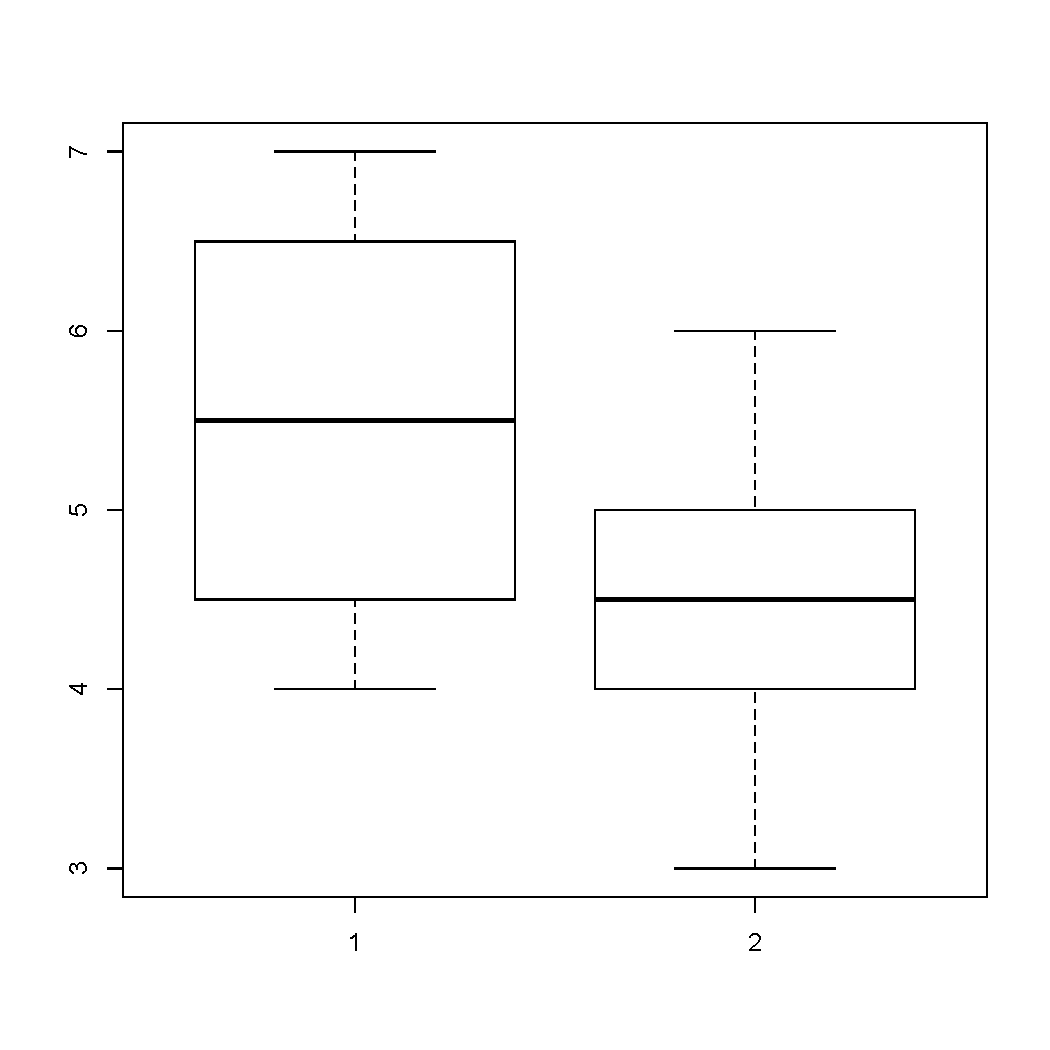
\includegraphics[width=.5\textwidth]{s1.pdf}
% section scenario_1 (end)

\section{Scenario 2} % (fold)
\label{sec:scenario_2}
\begin{description}
	\item[Hypothesis] 
		$H_0$: There is \textbf{no significant performance boost} after taking the drug.\\
		$H_1$: There is a \textbf{significant performance boost} after taking the drug.
	\item[Independent variable] Pills taken (either drug or placebo).
	\item[Dependent variable] Time needed to finish programming problem.
	\item[Population groups] \textbf{Two} groups of people, 7 taking the drug and 8 taking placebo. Noted as $X_1$ and $X_2$.
	\item[Mean] $\bar{X}_1=185.0571$, $\bar{X}_2=211.3375$
	\item[Variance] $s_1^2=444.3029$, $s_2^2=102.2998$
	\item[Pooled variance] $s_{\bar{X}_1-\bar{X}_2}^2=260.1474$
	\item[T value] $t = -3.1483, df = 13$
	\item[Significant difference?] $t = 3.1483 > \color{red}{2.16}$, reject $H_0$. \color{red}{Should be one-tail test, so 2.16 should be 1.771.}
\end{description}
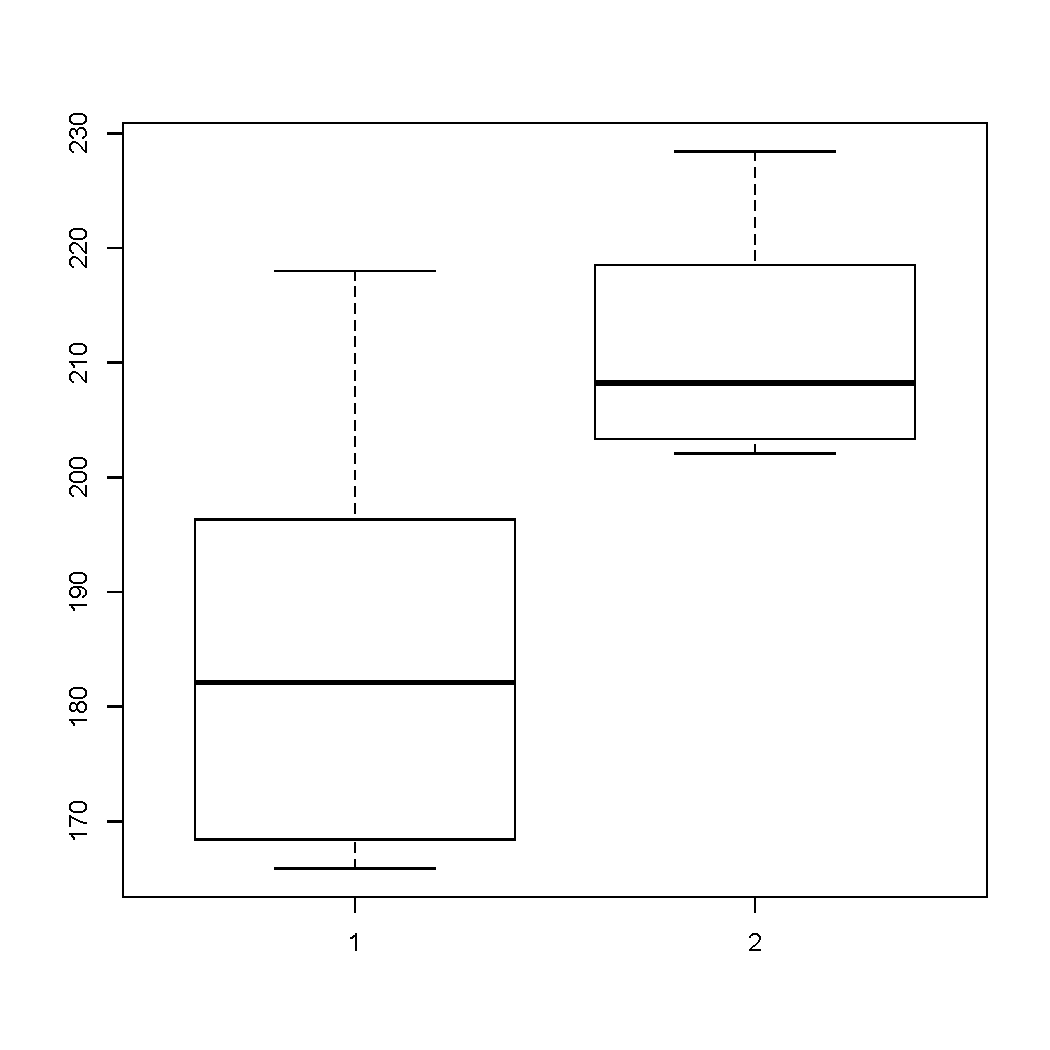
\includegraphics[width=.5\textwidth]{s2.pdf}
% section scenario_2 (end)

\section{Scenario 3} % (fold)
\label{sec:scenario_3}
\begin{description}
	\item[Hypothesis] 
		$H_0$: There is \textbf{no significant difference} in students' test performance after completing the education module.\\
		$H_1$: There is \textbf{significant difference} in students' test performance after completing the education module.
	\item[Independent variable] Time. Before and after the education.
	\item[Dependent variable] Students' test scores.
	\item[Population groups] \textbf{One} groups of 10 people. Scores before and after the education are noted as $X_1$ and $X_2$.
	\item[Mean] $\bar{X}_1=67$, $\bar{X}_2=76.4$
	\item[Variance] $s_1^2=176.8889$, $s_2^2=97.82222$
	\item[Pooled variance] $s_{\bar{X}_1-\bar{X}_2}^2=137.3556$
	\item[T value] $t = -3.1096, df = 9$
	\item[Significant difference?] $t = 3.1096 > 1.833$, reject $H_0$.
\end{description}
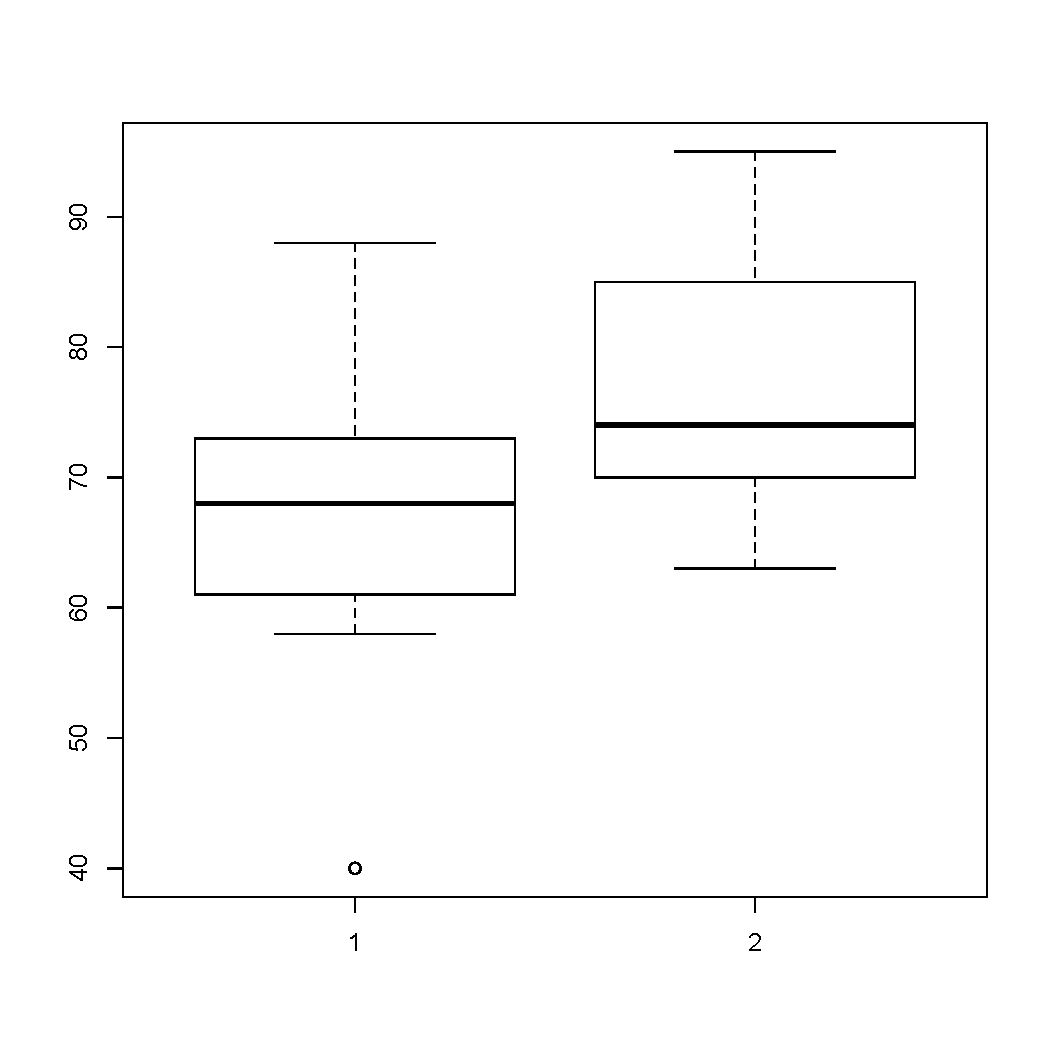
\includegraphics[width=.5\textwidth]{s3.pdf}
% section scenario_3 (end)

\section{Scenario 4} % (fold)
\label{sec:scenario_4}

% section scenario_4 (end)

\section{Interfaces A \& B} % (fold)
\label{sec:interfaces_a_&_b}
\begin{description}
	\item[Hypothesis] 
		$H_0$: There is \textbf{no significant difference} in time consumptions finishing a certain task between interface A and B.\\
		$H_1$: There is \textbf{significant difference} in time consumptions finishing a certain task between interface A and B.
	\item[Independent variable] Interface used.
	\item[Dependent variable] Task time.
	\item[Population groups] \textbf{Two} groups of people, each consists of 11. Noted as $X_1$ and $X_2$.
	\item[Mean] $\bar{X}_1=13.67273$, $\bar{X}_2=12.68182$
	\item[Variance] $s_1^2=11.58418$, $s_2^2=7.229636$
	\item[Pooled variance] $s_{\bar{X}_1-\bar{X}_2}^2=9.406909$
	\item[T value] $t = 0.7577, df = 20$
	\item[Significant difference?] $t = 0.7577 < 2.086$, do not reject $H_0$.
\end{description}
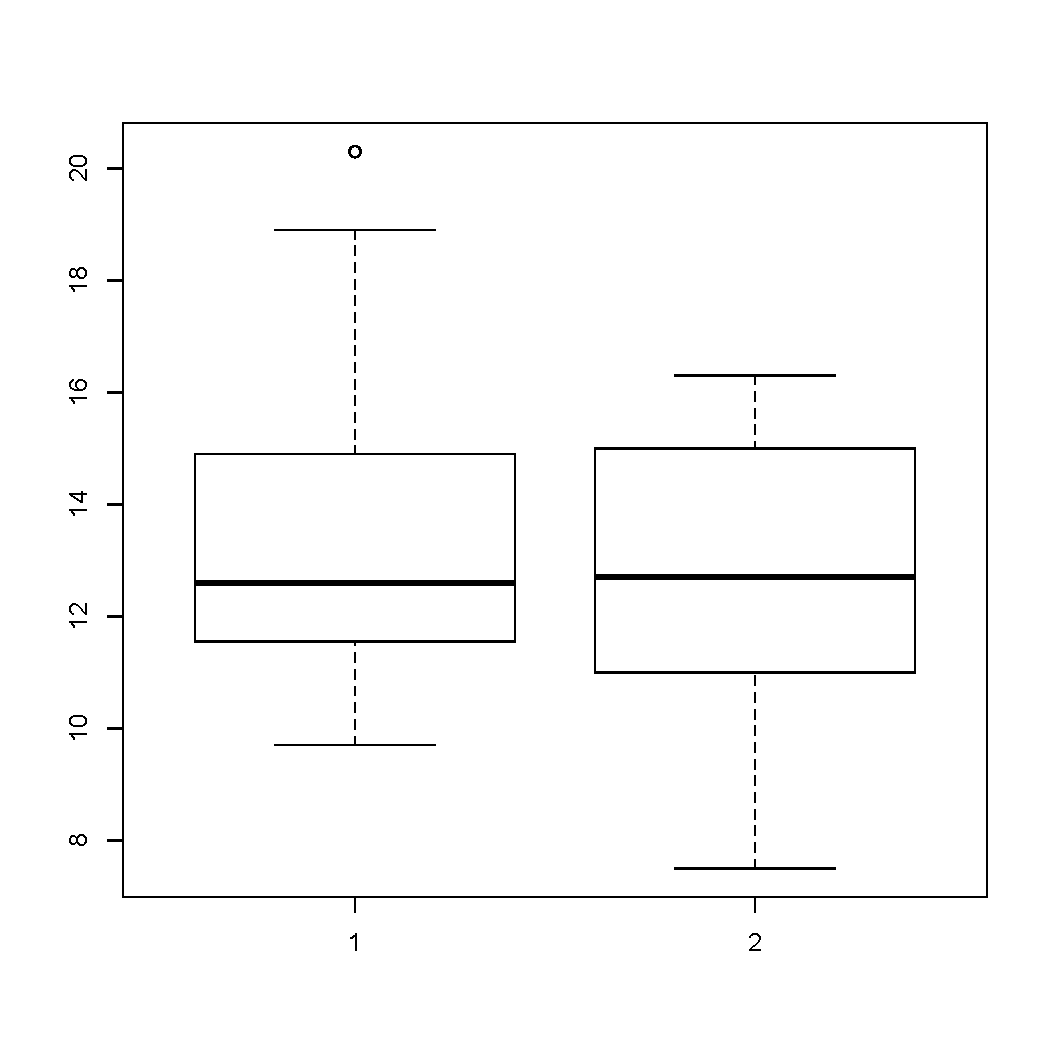
\includegraphics[width=.5\textwidth]{interface.pdf}
% section interfaces_a_&_b (end)

\section{Manual Typewriter vs Electric Typewriter} % (fold)
\label{sec:typewriter}
\begin{description}
	\item[Hypothesis] 
		$H_0$: There is \textbf{no significant difference} in average words per minute with manual typewriter or with electric typewriter.\\
		$H_1$: The average words per minute with manual typewriter is \textbf{significantly less} than that of electric typewriter.
	\item[Independent variable] Type of typewriter.
	\item[Dependent variable] Words per minute typed.
	\item[Population groups] \textbf{One} groups of 11 people. Words per minute with manual/electric typewriter noted as $X_1$ and $X_2$.
	\item[Mean] $\bar{X}_1=32.72727$, $\bar{X}_2=37$
	\item[Variance] $s_1^2=20.41818$, $s_2^2=19.8$
	\item[Pooled variance] $s_{\bar{X}_1-\bar{X}_2}^2=20.10909$
	\item[T value] $t = -5.875, df = 10$
	\item[Significant difference?] $t = 5.875 > 1.812$, reject $H_0$.
\end{description}
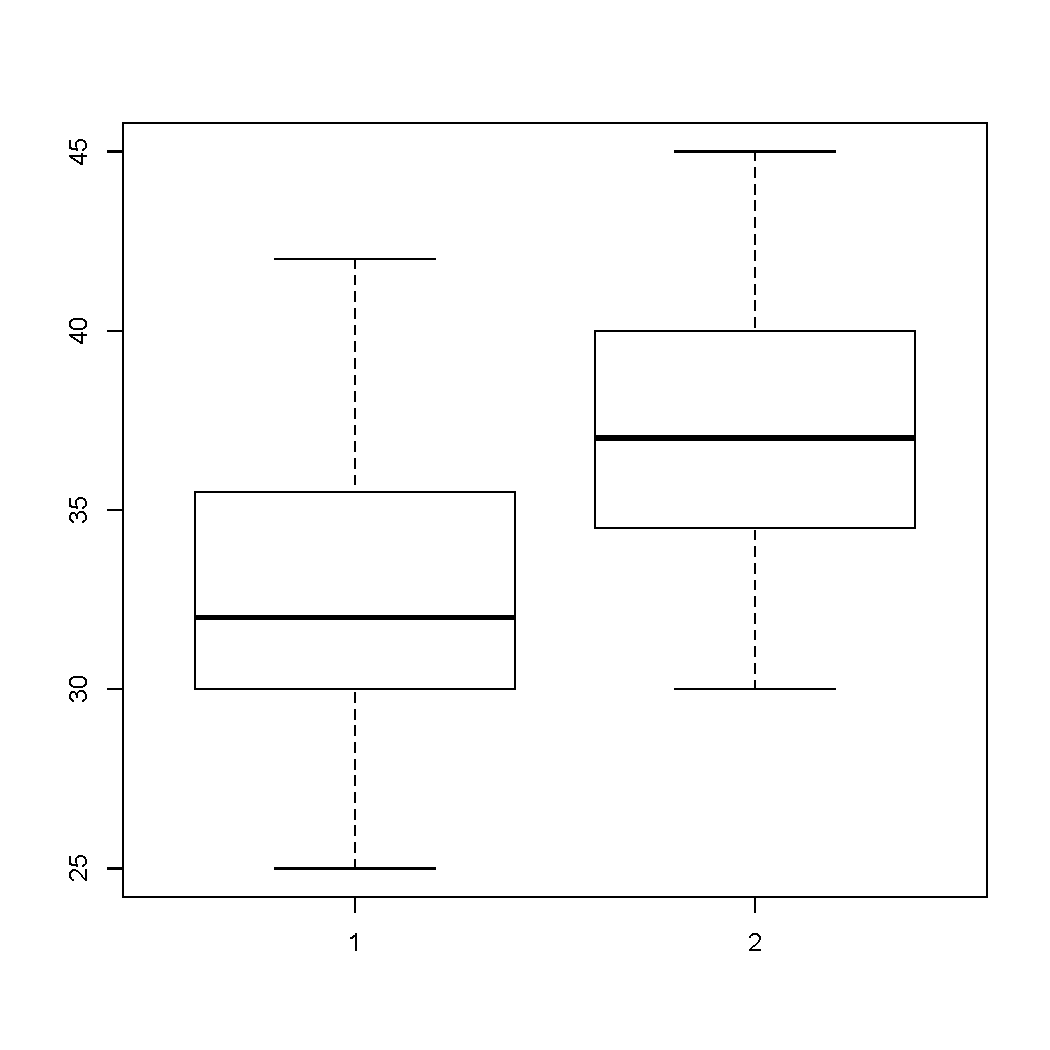
\includegraphics[width=.5\textwidth]{typewriter.pdf}
% section typewriter (end)

\end{document}